%------------------------------------------------------------------------------
% CV in Latex
% Author : Charles Rambo
% Based off of: https://github.com/sb2nov/resume and Jake's Resume on Overleaf
% Most recently updated version may be found at https://github.com/fizixmastr 
% License : MIT
%------------------------------------------------------------------------------

\documentclass[A4,11pt]{article}
%\documentclass[letterpaper,11pt]{article} %For use in US
\usepackage{latexsym}
\usepackage[empty]{fullpage}
\usepackage{titlesec}
\usepackage{marvosym}
\usepackage[usenames,dvipsnames]{color}
\usepackage{verbatim}
\usepackage{enumitem}
\usepackage[hidelinks]{hyperref}
\usepackage[english]{babel}
\usepackage{tabularx}
\usepackage{tikz}
\usepackage{fontawesome}
\input{glyphtounicode}

\begin{comment}
I am by no means a professional when it comes to the CV's/resumes, I have
received various trainings on how to write a CV and resume from my high 
school, as well as the Austin College and University of Eastern Finland's
career counseling departments. As I intend to share my CV as a template, I 
feel that it is my responsibility to provide explanations of my work.
\end{comment}


%-----FONT OPTIONS-------------------------------------------------------------
\begin{comment}
The font of the document will impact not just how readable it is, but how it is
perceived. In the "The Craft of Scientific Writing" by Michael Alley, shares a
common fonts for publication as well as their use. I have chosen to use
Palatino for its legibility, some others are given below. There is far too much
about typography to discus here. Note: serif fonts have short projecting
strokes, sans-serif fonts are sans (without) these strokes.
\end{comment}


% serif
 \usepackage{palatino}
% \usepackage{times} %This is the default as well
% \usepackage{charter}

% sans-serif
% \usepackage{helvet}
% \usepackage[sfdefault]{noto-sans}
% \usepackage[default]{sourcesanspro}

%-----PAGE SETUP---------------------------------------------------------------

% Adjust margins
\addtolength{\oddsidemargin}{-1cm}
\addtolength{\evensidemargin}{-1cm}
\addtolength{\textwidth}{2cm}
\addtolength{\topmargin}{-1cm}
\addtolength{\textheight}{2cm}

% Margins for US Letter size
%\addtolength{\oddsidemargin}{-0.5in}
%\addtolength{\evensidemargin}{-0.5in}
%\addtolength{\textwidth}{1in}
%\addtolength{\topmargin}{-.5in}
%\addtolength{\textheight}{1.0in}

\urlstyle{same}

\raggedbottom
\raggedright
\setlength{\tabcolsep}{0cm}

% Sections formatting
\titleformat{\section}{
  \vspace{-4pt}\scshape\raggedright\large
}{}{0em}{}[\color{black}\titlerule \vspace{-5pt}]

% Ensure that .pdf is machine readable/ATS parsable
\pdfgentounicode=1

%-----CUSTOM COMMANDS FOR FORMATTING SECTIONS----------------------------------
\newcommand{\CVItem}[1]{
  \item\small{
    {#1 \vspace{-2pt}}
  }
}

\newcommand{\CVSubheading}[4]{
  \vspace{-2pt}\item
    \begin{tabular*}{0.97\textwidth}[t]{l@{\extracolsep{\fill}}r}
      \textbf{#1} & #2 \\
      \small#3 & \small #4 \\
    \end{tabular*}\vspace{-7pt}
}

\newcommand{\CVSubSubheading}[2]{
    \item
    \begin{tabular*}{0.97\textwidth}{l@{\extracolsep{\fill}}r}
      \text{\small#1} & \text{\small #2} \\
    \end{tabular*}\vspace{-7pt}
}

\newcommand{\CVSubItem}[1]{\CVItem{#1}\vspace{-4pt}}

\renewcommand\labelitemii{$\vcenter{\hbox{\tiny$\bullet$}}$}

\newcommand{\CVSubHeadingListStart}{\begin{itemize}[leftmargin=0.5cm, label={}]}
% \newcommand{\resumeSubHeadingListStart}{\begin{itemize}[leftmargin=0.15in, label={}]} % Uncomment for US
\newcommand{\CVSubHeadingListEnd}{\end{itemize}}
\newcommand{\CVItemListStart}{\begin{itemize}}
\newcommand{\CVItemListEnd}{\end{itemize}\vspace{-5pt}}

%------------------------------------------------------------------------------
% CV STARTS HERE  %
%------------------------------------------------------------------------------
\begin{document}

%-----HEADING------------------------------------------------------------------
\begin{comment}
In Europe it is common to include a picture of ones self in the CV. Select
which heading appropriate for the document you are creating.
\end{comment}

% \begin{minipage}[c]{0.05\textwidth}
% \-\
% \end{minipage}
% \begin{minipage}[c]{0.2\textwidth}
% \begin{tikzpicture}
%     \clip (0,0) circle (1.75cm);
%     \node at (0,-.7) {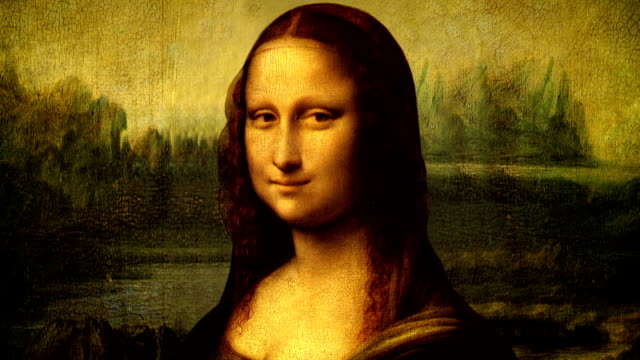
\includegraphics[width = 9cm]{portrait}}; 
%     % if necessary the picture may be moved by changing the at (coordinates)
%     % width defines the 'zoom' of the picture
% \end{tikzpicture}
% \hfill\vline\hfill
% \end{minipage}
% \begin{minipage}[c]{0.4\textwidth}
%     \textbf{\Huge \scshape{Charles Rambo}} \\ \vspace{1pt} 
%     % \scshape sets small capital letters, remove if desired
%     \small{+1 123-456-7890} \\
%     \href{mailto:you@provider.com}{\underline{you@provider.com}}\\
%     % Be sure to use a professional *personal* email address
%     \href{https://www.linkedin.com/in/charles-rambo/}{\underline{linkedin.com/in/charles-rambo}} \\
%     % you should adjust you linked in profile name to be professional and recognizable
%     \href{https://github.com/fizixmastr}{\underline{github.com/fizixmastr}}
% \end{minipage}

% Without picture
\begin{center}
  \textbf{\huge Cyris Tseng (Yu-Chun, Tseng)} \\ \vspace{1pt} %\scshape sets small capital letters, remove if desired
  \vspace{3mm}
  \faGlobe{ \href{https://blog.eevee.tw}{blog.eevee.tw}} $|$
  \faMobile{ \small (+886) 975-428-633} $|$
  \faEnvelopeO{ \href{mailto:cyris.tseng@gmail.com}{cyris.tseng@gmail.com}} $|$
  % Be sure to use a professional *personal* email address
  % you should adjust you linked in profile name to be professional and recognizable
  \faGithub{ \href{https://github.com/yctseng1227}{github.com/yctseng1227}} \\
  \textbf{Languages}{: Chinese (Native language), English} \\
\end{center}


\begin{comment}
This CV was written for specifically for positions I was applying for in
academia, and then modified to be a template.

A standard CV is about two pages long where as a resume in the US is one page.
sections can be added and removed here with this in mind. In my experience, 
education, and applicable work experience and skills are the most import things
to include on a resume. For a CV the Europass CV suggests the categories: Work
Experience, Education and Training, Language Skills, Digital Skills,
Communication and Interpersonal Skills, Conferences and Seminars, Creative Works
Driver's License, Hobbies and Interests, Honors and Awards, Management and
Leadership Skills, Networks and Memberships, Organizational Skills, Projects,
Publications, Recommendations, Social and Political Activities, Volunteering.

Your goal is to convey a who, what , when, where, why for every item you share. 
The who is obviously you, but I believe the rest should be done in that order.
For example below. An employer cares most about the degree held and typically 
less about the institution or where it is located (This is still good 
information though). Whatever order you choose be consistent throughout.
\end{comment}

%-----EDUCATION----------------------------------------------------------------
\section{Education}
  \CVSubHeadingListStart
%    \CVSubheading % Example
%      {Degree Achieved}{Years of Study}
%      {Institution of Study}{Where it is located}
    \CVSubheading
      {M.S. in Computer Science and Engineering $|$ \emph{\small{Information Security}}}{Aug. 2019 -- July 2022 (expected)}
      {National Sun Yat-sen University (NSYSU)}{Kaohsiung, Taiwan}
    \CVSubheading
      {B.S. in Computer Science and Information Engineering}{Aug. 2016 -- July 2018}
      {National University of Kaohsiung (NUK)}{Kaohsiung, Taiwan}
  \CVSubHeadingListEnd

%-----WORK EXPERIENCE----------------------------------------------------------
\begin{comment}
  try to briefly explain what you did and why it is relevant to the position you
  are seeking
  \end{comment}
  
  \section{Experience}
    \CVSubHeadingListStart
  %    \CVSubheading %Example
  %      {What you did}{When you worked there}
  %      {Who you worked for}{Where they are located}
  %      \CVItemListStart
  %        \CVItem{Why it is important to this employer}
  %      \CVItemListEnd
      \CVSubheading
        {Penetration Test Intern}{May 2020 -- Aug. 2020}
        {National Center for Cyber Security Technology}{Tainan, Taiwan}
        \CVItemListStart
          \CVItem{Executed penetration tests on public agencies' external systems}
          \CVItem{Explored vulnerabilities and reported the relevant agencies}
          \CVItem{Received performance bonus based on results}
        \CVItemListEnd
      \CVSubheading
        {Club's Teaching Assistant}{Sep. 2019 -- Aug. 2021}
        {Information Security Club, NSYSU}{Kaohsiung, Taiwan}
        \CVItemListStart
          \CVItem{Aided and provided resources during the start-up period}
          \CVItem{Acted as a course assistant to guide members in learning and solving problems}
          \CVItem{Assisted lecturer with problem testing and writing write-ups}
        \CVItemListEnd
      \CVSubheading
        {Club's Founding President}{Sep. 2017 -- Aug. 2018}
        {Competitive Programming Club, NUK}{Kaohsiung, Taiwan}
        \CVItemListStart
          \CVItem{Founded and promoted the club since the algorithm competition was not popular in the department}
          \CVItem{Acted as a lecturer during the startup period, the average attendance rate of the club members was over 80\%}
          \CVItem{Leaded members to participate in competitions in other cities}
        \CVItemListEnd
    \CVSubHeadingListEnd

%-----PROJECTS AND RESEARCH----------------------------------------------------
\begin{comment}
  Ideally the title of the work should speak for what it is. However if you feel
  like you should explain more about why the project is applicable to this job,
  use item list as is shown in the work experience section.
  \end{comment}
  
  \section{Projects}
    \CVSubHeadingListStart
  % %    \CVSubheading
  % %      {Title of Work}{When it was done}
  % %      {Institution you worked with}{unused}
      % \CVSubheading
      %   {Botnet Detection Based on the Behaviors of DNS over TLS Queries}{Summer 2022}
      %   {National Sun Yat-sen University}{}
      \CVSubheading
        {EVERCTF: An automatic deployment CTF platform $|$ \emph{\small{Docker, Jenkins}}}{Spring 2021}
        {National Sun Yat-sen University}{}
    \CVSubHeadingListEnd

%-----CONFERENCES AND PRESENTATIONS--------------------------------------------
\begin{comment}
Again the title should have already been enough, but if it is necessary to add
descriptions maintain the consistency from prior sections
\end{comment}

% \section{Conferences and Presentations}
%   \CVSubHeadingListStart
%    \CVSubheading % Example
%      {Work Presented}{When}
%      {Occasion}{}
  %   \CVSubheading
  %     {Cloud Gaming System and Security}{August 2021}
  %     {Cryptology and Information Security Conference}{}
  % \CVSubHeadingListEnd

%-----HONORS AND AWARDS--------------------------------------------------------
\section{Honors}
  \CVSubHeadingListStart
% %    \CVSubheading %Example
% %      {What}{When}
% %      {Short Description}{}
    \CVSubheading
      {CISC Personal CTF Outstanding Award}{September 2020}
      {Jeopardy-style CTF focusing on reverse, web security, pwn, cryptography, and miscellaneous}{}
    \CVSubheading
      {T-Cat Cup Information Security Competitive (Colleges Group) 1st Place}{May 2020}
      {Mainly with web security, cryptology and forensics security challenge}{}
    \CVSubheading
      {ITSA Annual Collegiate Programming Contest Honorable Mention}{May 2018}
      {An annual competitive programming competition among the universities in Taiwan}{}
    \CVSubheading
      {ACM-ICPC Asia Hua-Lien Regional Contest Honorable Mention}{November 2017}
      {An annual competitive programming competition among the universities in Asia}{}
  \CVSubHeadingListEnd

%-----CERTIFICATE--------------------------------------------------------------
\section{Certificate}
  \CVSubHeadingListStart
% %    \CVSubheading %Example
% %      {What}{When}
% %      {Short Description}{}
    \CVSubheading
      {Collegiate Programming Examination Rank: 1.1\% (26/2420)}{March 2019}
      {ACM-ICPC Contest Council for Taiwan}{}      
  \CVSubHeadingListEnd

%-----TEACHING EXPERIENCE------------------------------------------------------
\begin{comment}
  Section is here as it applied to my application for positions in academia. 
  Remember to tailor the resume for to the position.
  \end{comment}
  
  % \section{Teaching Experience}
  %   \CVSubHeadingListStart
  % % %    \CVSubheading
  % % %      {What}{When}
  % % %      {School}{Where}
  %     \CVSubheading
  %       {Things about Network Security (2 Hours Teaching)}{September 2021}
  %       {The Affiliated Senior High School of National Kaohsiung Normal University}{Kaohsiung, Taiwan}
  %     \CVSubheading
  %       {Basic Web Security Training (3 Hours Teaching)}{September 2020}
  %       {Cryptology and Information Security Conference}{Kaohsiung, Taiwan}
  %   \CVSubHeadingListEnd

%-----COMMUNITY INVOLVEMENT----------------------------------------------------
% \section{Community Involvement}
%   \CVSubHeadingListStart
% %    \CVSubheading %Example
% %      {What you did}{When you worked there}
% %      {Who you worked for}{Where they are located}
  %   \CVSubheading
  %     {Trainees}{Summer 2020}
  %     {Advanced Information Security Summer School (AIS3)}{Taipei, Taiwan}
  % \CVSubHeadingListEnd

%-----SKILLS-------------------------------------------------------------------
\begin{comment}
This section is compressed from the various skills sections that Euro CV
recommends.
\end{comment}

\section{Skills}
 \begin{itemize}[leftmargin=0.5cm, label={}]
    \small{\item{
      % \textbf{Had better or finished works}{: C/C++, Python, Bash script} \\
      % \textbf{Had semi-finished works}{: PHP, SQL, Jenkins, Golang} \\
      % \textbf{Learned only or had simple samples}{: C\#, Java, MATLAB} \\
      % \textbf{Others}{: Docker, Git, \LaTeX, Markdown}
      \textbf{Programming}{: C/C++, Python, Bash Script, PHP, SQL, Golang} \\
      \textbf{Technologies}{: Linux, Git, Docker, Jenkins, Github Actions} \\
    }}
 \end{itemize}
    
%------------------------------------------------------------------------------
\end{document}